\begin{titlepage}

\chapter{Diseño}

% Arquitectura del software, diagramas de clases, diagramas de secuencia

\section{Arquitectura del software}

A continuación muestro un esquema equivalente a la arquitectura general del software.\newline

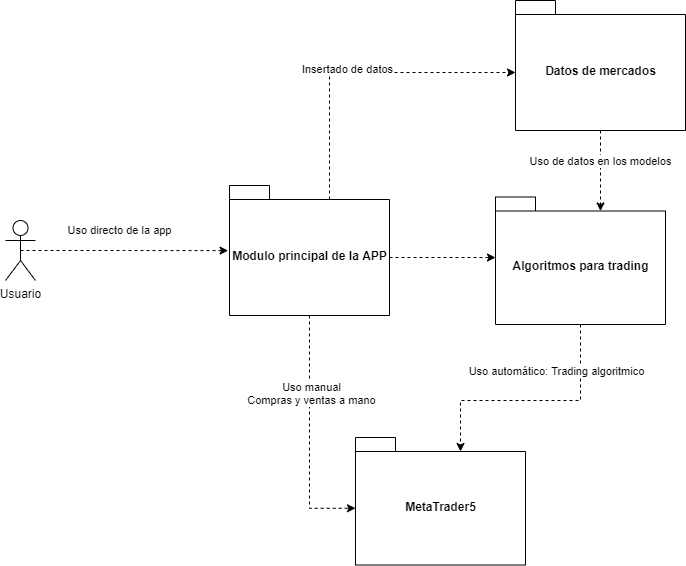
\includegraphics[width=1\textwidth]{imagenes/arquitectura general.png}\\[0.1cm]

Como resumen, en el esquema podemos ver cuál es la idea principal del proyecto. El usuario de la aplicación (véase punto 2.2, segundo implicado) será el que haga un uso directo de la interfaz de la aplicación. A continuación presento cada uno de los módulos con sus funciones y demás utilidades:\newline

\begin{itemize}
	\item \textbf{Módulo principal de la APP}: este módulo se corresponderá con el controlador principal del software. Será usado por el usuario a través de una interfaz escrita en Django y se comunicará con el resto de módulos directamente.
	\item \textbf{Datos de mercados}: este módulo se corresponderá con la base de datos y las operaciones que hagamos con dichos datos (insertado de datos, adaptaciones a cada algoritmo, etc.) Será usado por la interfaz principal de la aplicación y mandará los inputs a los algoritmos.\newline
	\item \textbf{Algoritmos para trading o backend}: se corresponde con el backend o código fuente de la aplicación. Aquí se encontrará cada uno de los algoritmos que usemos para trading algorítmico. Recibe datos de la BBDD y se comunica con el módulo de MetaTrader5 para indicar cada una de las operaciones decididas y obtener información en tiempo real.
	\item \textbf{MetaTrader5}: Módulo externo de la aplicación, se usará para mandar órdenes de operaciones y recibir resultados e información en tiempo real.
\end{itemize}

El software estará escrito en Python, usando Django como Framework para la interfaz web.
% COMPLETAR CON MAS DETALLES DE HERRAMIENTAS

\end{titlepage}